\documentclass[a4paper,12pt]{article}

\author{}
\date{}
\title{Two-dimensional Filtration of Nitrogen and Pentane
\(\left( C_5 H_{12} \right) \)}

\usepackage[margin=0.9in]{geometry}
\usepackage{graphicx}
\usepackage{float}
\usepackage{textcomp}
\usepackage{amsmath, amssymb}
\usepackage{siunitx}
\usepackage{subcaption}
\usepackage{multirow}
\usepackage{bm}
\usepackage{ulem}
\usepackage{xcolor}

\definecolor{grey}{HTML}{737373}
\definecolor{red}{HTML}{d9343f}
\definecolor{green}{HTML}{2e8a07}

\begin{document}
\maketitle

\section{Mathematical model}

Darcy's law:
\begin{equation}
    \bm{v}_i = -\frac{1}{\mu_i} \hat K \cdot f_\alpha (s)
    \cdot \nabla P
\end{equation}
where \(\hat K\), the specific permeability.
It depends only on the geometry of the medium.
We assume isotropy of space, so K is a scalar.
\(\mu\) is the dynamic viscosity.

\(i\) - component.

\(\alpha\) - phase. (If we had multiple phases, then
it would be \(f_\alpha\))

As an approximation, \(f_\alpha (s) = s^2\) for the first 
component, and \(f_\alpha (s) = (1 - s)^2\) for the second.

The continuity equation for each component becomes:
\begin{equation}
    \varphi \frac{\partial \rho_i}{\partial t}
    + div (\rho_i \bm{v}_i) = 0
\end{equation}
where \(\rho_i = \frac{m_i}{V}\).

We use the Tait equation to relate liquid density to pressure:
\begin{equation}
    \frac{\hat{\rho} - \rho_0}{\hat{\rho}} = C \log_{10}
    \frac{B + P}{B + P_0}
\end{equation}
where \(C = 0.2105\),
\(\rho_0 = \frac{1}{67.28 \frac{m^3}{mol}}\),
\(P_0 = 0.1 MPa\), \(B = 35MPa\),
in the case of \(C_5H_{12}\).

Ideal gas equation of state:

\begin{equation}
    P = \frac{RT}{M} \hat{\rho}
\end{equation}
\section{Discretization Scheme}

\subsection{Staggered Grid}

\begin{figure}[H]
    \centering
    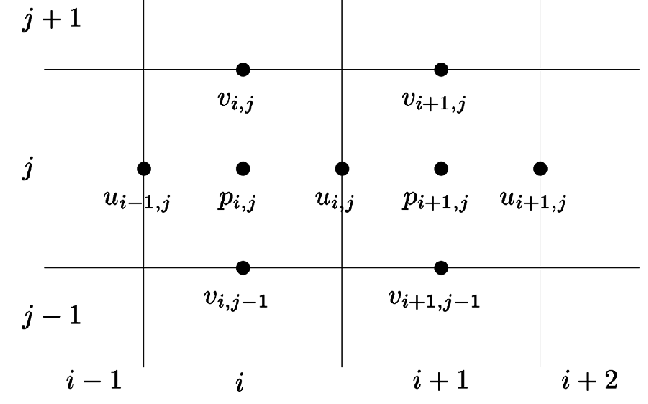
\includegraphics[width=0.5\textwidth]{img/staggered-grid.png}
    \caption{Staggered Grid}
\end{figure}

\begin{figure}[H]
    \centering
    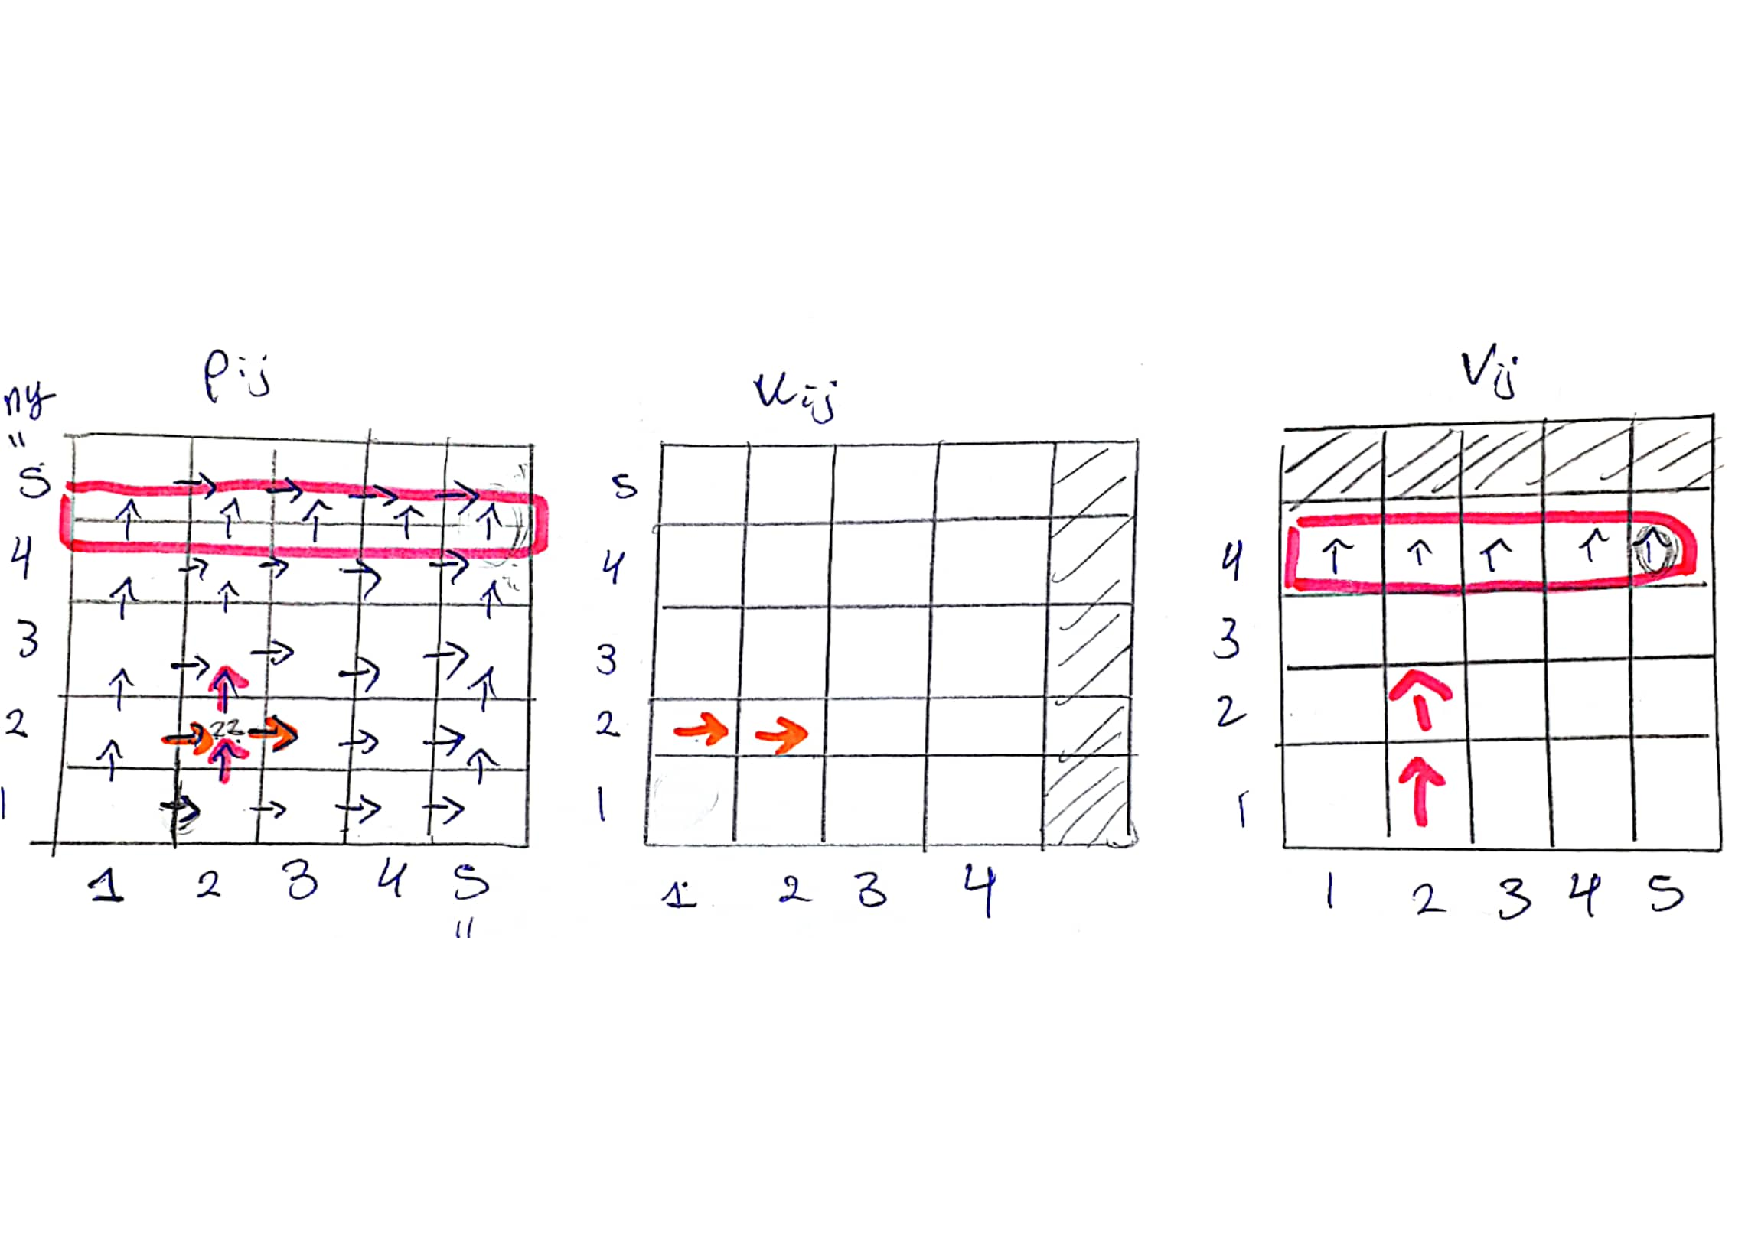
\includegraphics[width=\textwidth]{img/staggered-grid2.pdf}
    \caption{Staggered Grid Dimensions}
\end{figure}

\subsection{Fluxes}


We extrapolate the densities to where velocities are defined as:

\[
    \rho_{i + \frac{1}{2}, j} = \frac{\rho_{i, j} +
    \rho_{i + 1, j}}{2}
\] 

\[
    \rho_{i, j + \frac{1}{2}} = \frac{\rho_{i, j} +
    \rho_{i, j + 1}}{2}
\] 

Flux along the x axis: \(\Phi_x\)
\[
    \Phi_{x, (i + \frac{1}{2}, j)} = u_{i + \frac{1}{2}, i} \cdot
    \rho_{i + \frac{1}{2}, i}
\] 

Flux along the y axis: \(\Phi_y\)
\[
    \Phi_{y, (i, j + \frac{1}{2})} = v_{i, j + \frac{1}{2}} \cdot
    \rho_{i, j + \frac{1}{2}}
\] 

\subsection{Continuity Equation}

\[
\varphi \frac{\partial \rho}{\partial t}
+ div \Phi = 0
\] 

\[
\varphi \frac{\partial \rho}{\partial t}
+ \frac{\partial \Phi_x}{\partial x}
+ \frac{\partial \Phi_y}{\partial y} = 0
\] 

\[
\varphi \frac{\rho^{n + 1}_{i, j} - \rho^n_{i, j}}{\Delta t}
+ \frac{\Phi_{x, i - \frac{1}{2}, j}^n -
        \Phi_{x, i + \frac{1}{2},j}^n}{\Delta x}
+ \frac{\Phi_{i, j + \frac{1}{2}}^n - \Phi_{y, i, j - \frac{1}{2}}^n}
{\Delta y} = 0
\] 

\subsection{Darcy's Law}

\[
    u_{i + \frac{1}{2} , j}^n = -\frac{K}{\mu} f_\alpha (s_{i, j}^n)
    \frac{P_{i + 1, j}^n - P_{i, j}^n}{\Delta x} \\
\] 

\[
    v_{i, j + \frac{1}{2}}^n = -\frac{K}{\mu} f_\alpha(s_{i, j}^n)
    \frac{P_{i, j + 1}^n - P_{i, j}^n}{\Delta y}
\] 

% \subsubsection{BC}
% 
% \[
%     v_{i, 1}^n = -\frac{K}{\mu} f_\alpha(s_{i, 1}^n)
%     \frac{-3 P_{i, 1}^n + 4 P_{i, 2}^n - P_{i, 3}^n }
%     {2 \Delta x} \qquad \text{(Inlet)}
% \] 
% 
% \[
%     v_{i, ny}^n = -\frac{K}{\mu} f_\alpha(s_{i, ny}^n)
%     \frac{-3 P_{i, ny}^n + 4 P_{i, ny - 1}^n
%     - P_{i, ny - 2}^n }{(-2 \Delta x)}
%     \qquad \text{(Outlet)}
% \] 

\subsection{Predictor-Corrector}

\begin{enumerate}
    \item Predictor
        \begin{enumerate}
            \item Continuity Equation
\begin{align*}
    \tilde \rho_{i, j}^{n+1} &= \rho_{i, j}^n
    - \frac{\Delta t}{\varphi} \left( 
  \frac{\Phi_{x, i - \frac{1}{2}, j}^n -
        \Phi_{x, i + \frac{1}{2},j}^n}{\Delta x}
+ \frac{\Phi_{i, j + \frac{1}{2}}^n - \Phi_{y, i, j - \frac{1}{2}}^n}
{\Delta y}
\right) \\
%                              &\left.+
%   \frac{u_{i+1, j} - u_{i-1,j}^n}{2\Delta x} \rho_{i,j}^n
% + \frac{v_{i, j+1}^n - v_{i,j-1}^n}{2\Delta y} \rho_{ij}^n
%     \right) \\
    \tilde \rho_{i, j}^{n + 1} &= \rho_{i, j}^n + F_\rho^n \Delta t 
\end{align*}

            \item Compute Pressure \(\tilde P^n\)
            \item Enforce boundary conditions for pressure,
                density, and saturation.

            \item Darcy's Law
\[
    \tilde u_{i + \frac{1}{2},j}^n = -\frac{K}{\mu}
    f_\alpha (\tilde s_{i, j}^n)
    \frac{\tilde P_{i + 1, j}^n - \tilde P_{i, j}^n}{\Delta x} \\
\] 

\[
    \tilde v_{i, j + \frac{1}{2}}^n = -\frac{K}{\mu}
    f_\alpha(\tilde s_{i, j}^n)
    \frac{\tilde P_{i, j + 1}^n - \tilde P_{i, j}^n}{\Delta y}
\] 
        \end{enumerate}

    \item Corrector
        \begin{enumerate}
            \item Continuity Equation

\[
    \tilde F^{n + 1} = -\frac{1}{\varphi} \left( 
        \frac{\tilde\Phi_{x, i - \frac{1}{2}, j}^{n + 1} -
        \tilde\Phi_{x, i + \frac{1}{2},j}^{n + 1}}{\Delta x}
        + \frac{\tilde\Phi_{i, j + \frac{1}{2}}^{n + 1}
        - \tilde\Phi_{y, i, j - \frac{1}{2}}^{n + 1}}{\Delta y}
    \right)
\]

\begin{align*}
    \rho_{i, j}^{n + 1} = \rho_{i, j}^n + \frac{F_\rho^n
    + \tilde F_\rho^{n+1} }{2} \Delta t
\end{align*}

            \item Compute Pressure \(P^n\)
            \item Enforce boundary conditions for pressure,
                density, and saturation.
            \item Darcy's Law
\[
    u_{i + \frac{1}{2}, j}^n = -\frac{K}{\mu} f_\alpha (s_{i, j}^n)
    \frac{P_{i + 1, j}^n - P_{i, j}^n}{\Delta x} \\
\] 

\[
    v_{i, j + \frac{1}{2}}^n = -\frac{K}{\mu} f_\alpha(s_{i, j}^n)
    \frac{P_{i, j + 1}^n - P_{i, j}^n}{\Delta y}
\] 
        \end{enumerate}
\end{enumerate}

\section{Boundary and Initial Conditions}
Check pluto notebook: src/BoundaryConditions.jl

Todo: update here.

% 
% On the first iteration, we set an initial
% pressure and molar composition.
% Then, we derive the velocities from the 
% pressure gradient using Darcy's law and the
% saturation from the densities
% and molar composition.
% 
% % All our BC are 2-nd order (thanks to ghost
% %     cells), except for the BC on velocity on the inlet
% % and outlet, which end up 1-st order.
% 
% \begin{figure}[H]
%     \centering
%     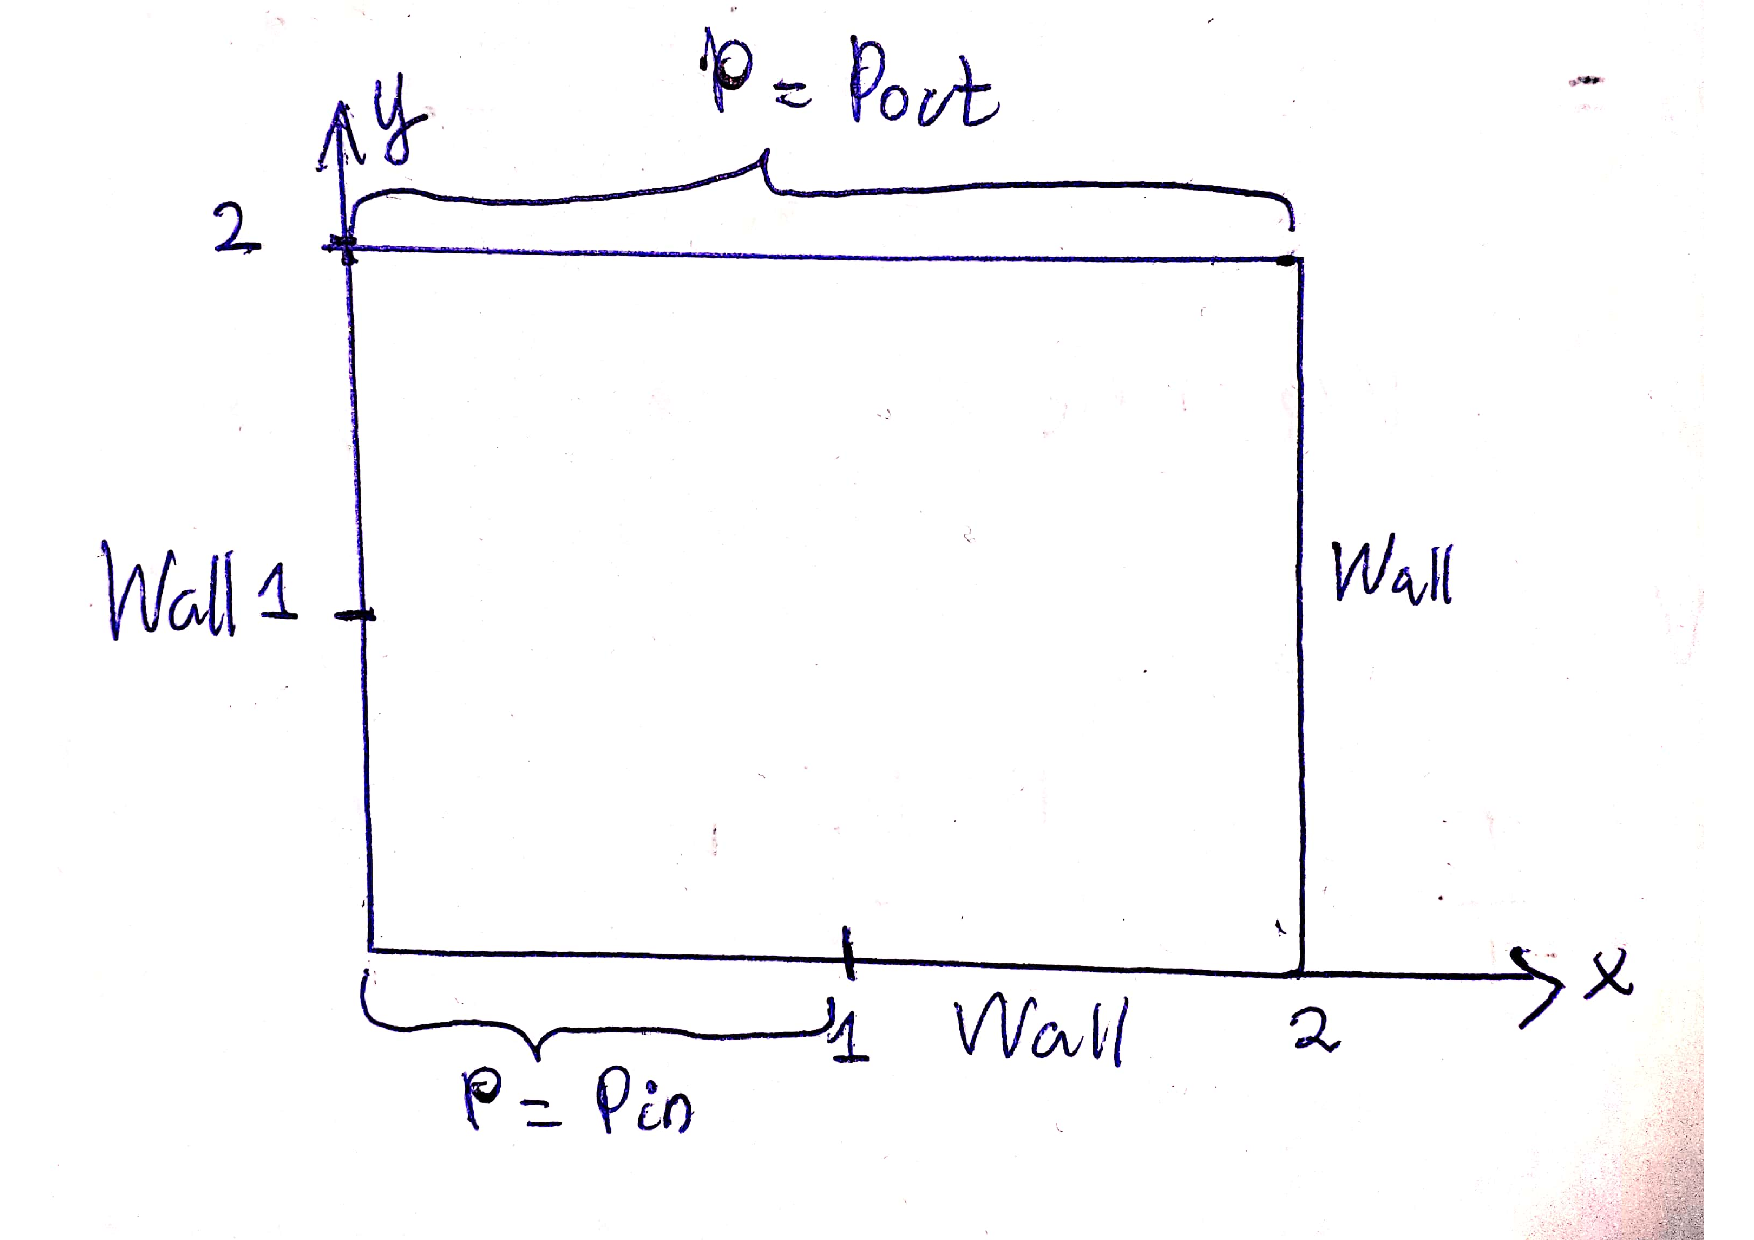
\includegraphics[width=0.5\textwidth]{img/diagram.pdf}
%     \caption{Boundary Conditions}
%     \label{fig:img-diagram-pdf}
% \end{figure}
% 
% \subsection{Pressure}
% 
% \textbf{BC:}
% 
% \[
% \begin{cases}
%     P = P_{in} &\text{at } y = 0
%     \text{ and } x \in [0, 1] \\
%     P = P_{out} &\text{at } y = 2 \\
%     \frac{\partial P}{\partial x} = 0 &\text{at }
%     x = 0, 2 \\
%     \frac{\partial P}{\partial y} = 0 &\text{at }
%     y = 0 \text{ and } x \in [1, 2]
% \end{cases}
% \] 
% 
% \textbf{IC:}
% 
% \[
% \begin{cases}
%     P = P_{out} &\text{at outlet} \\
%     P = P_{in}  &\text{at inlet} \\
%     P = P_0     &\text{everywhere else}
% \end{cases}
% \] 
% 
% % \subsection{Velocities}
% % 
% % \textbf{IC:} Darcy 2-nd order.
% % 
% % \textbf{BC:}
% % 
% % \[
% % \begin{cases}
% %     u = 0 &\text{at } x = 0, 2 \\
% %     v = 0 &\text{at } y = 0 \text{ and } x \in [1, 2] \\
% %     \text{Darcy (2-nd Order FD)}
% %           &\text{at } y = 2 \\
% %     \text{Darcy (2-nd Order FD)}
% %           &\text{at } y = 0
% %     \text{ and } x \in [0, 1]\\
% % \end{cases}
% % \] 
% 
% \subsection{Saturation}
%     Boundary condition on the inlet as the molar
%     composition \(\psi\):
%     \[
%         \frac{m_1}{m_2} = \frac{\psi}{1 - \psi}
%         \frac{M_1}{M_2}
%     \] 
%     where \(M_1\) and \(M_2\) represent the molar mass 
%     of each component.
% 
%     We can derive the densities from the equations of state,
%     then we can find the saturation.
% 
%     \[
%     \hat \rho_1 = \frac{m_1}{sV}, \qquad
%     \hat \rho_2 = \frac{m_2}{(1 - s)V}
%     \] 
% 
%     \[
%     \frac{\hat \rho_1}{\hat \rho_2} = \frac{m_1}{m_2}
%     \frac{1 - s}{s}
%     = \frac{\psi M_1}{(1 - \psi) M_2}\frac{1 - s}{s}
%     \] 
% 
%     \[
%         s = \left( 
%         \frac{\hat \rho_1 M_2(1 - \psi) }{\hat \rho_2 M_1 \psi}
%     + 1 \right)^{-1}
%     \] 
% 
%     \subsubsection{Outlet}
% 
%     \[
%     \frac{\partial s}{\partial \bm{n}} = 0 
%     \] 
% 
%     \subsubsection{Inlet}
% 
%     \begin{figure}[H]
%         \centering
%         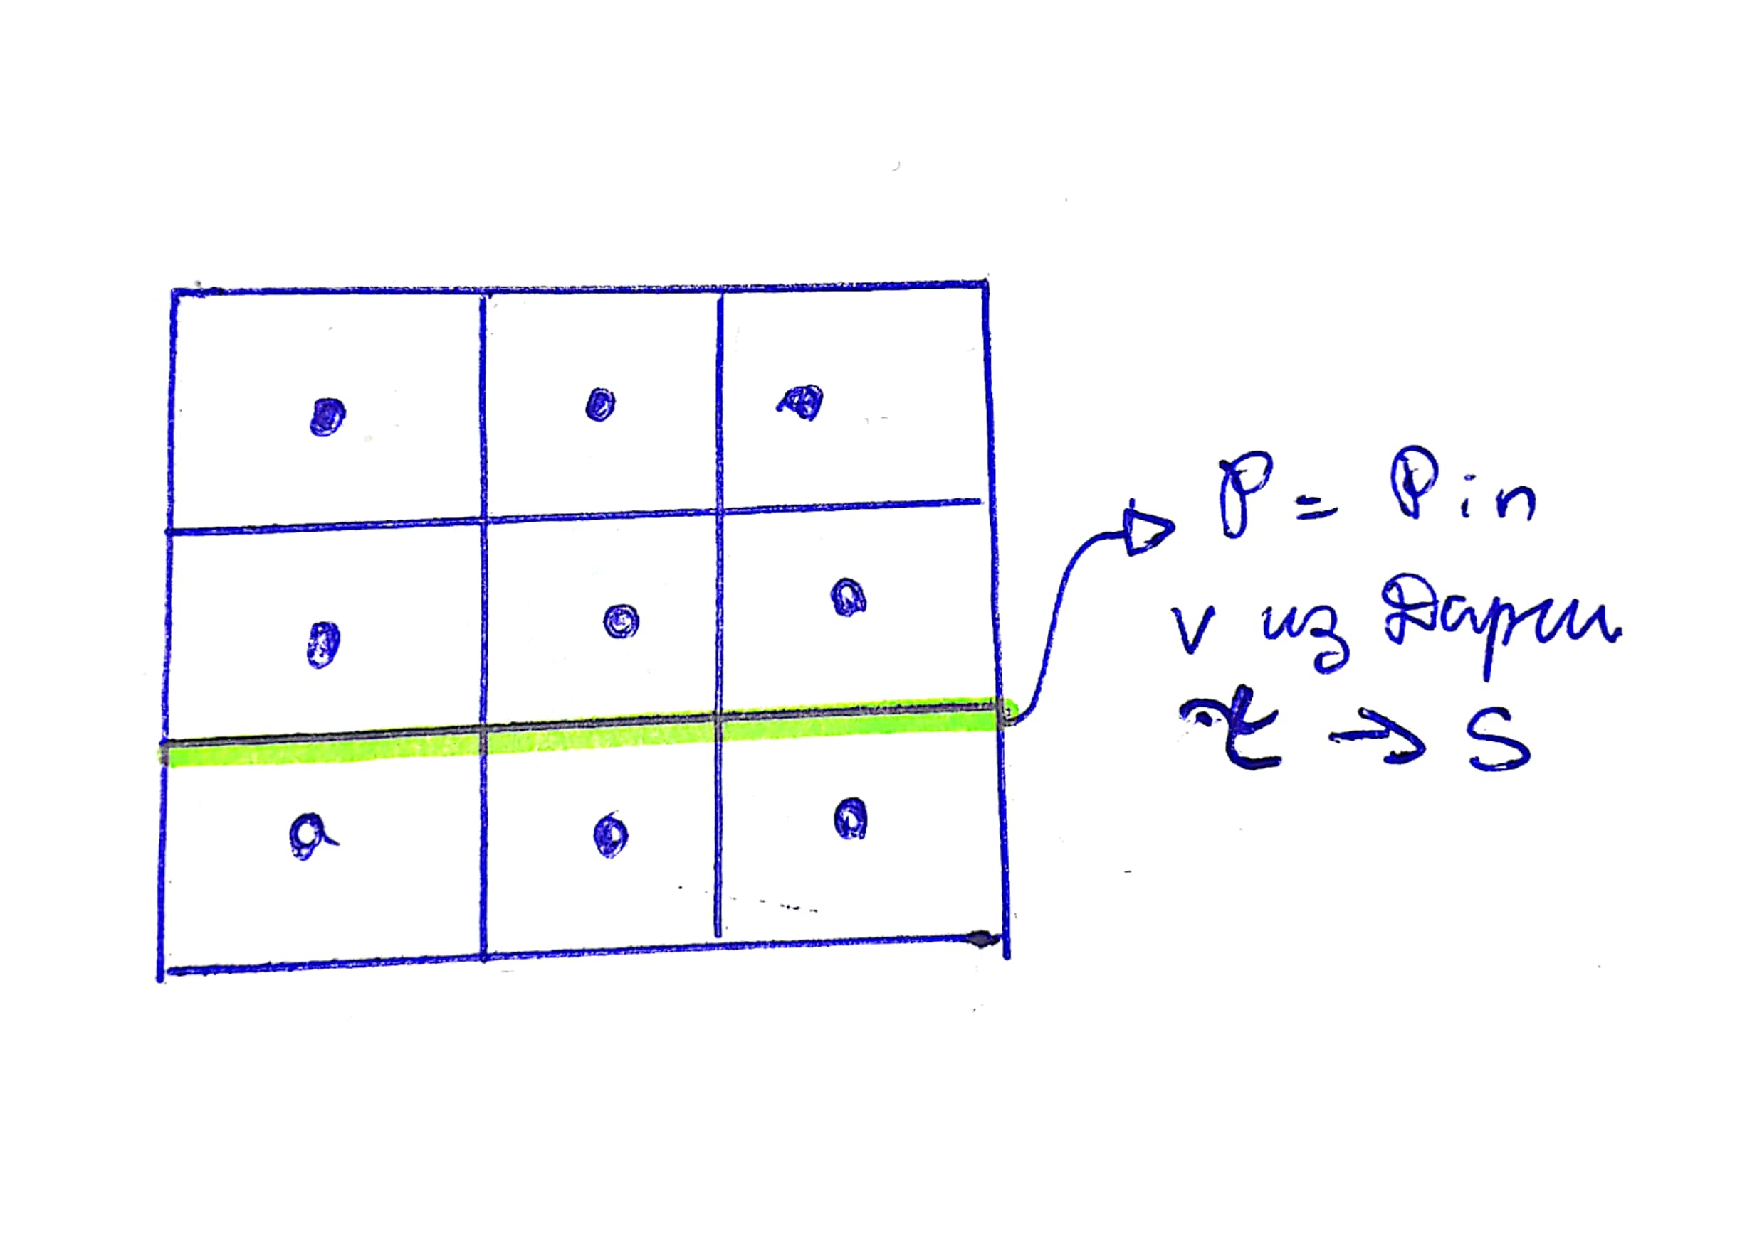
\includegraphics[width=0.6\textwidth]{img/inlet.pdf}
%         \caption{Boundary Conditions on the inlet.}
%     \end{figure}
% 
%     \[
%         \hat{\rho}_{\partial \Omega} = \frac{
%           \hat{\rho}_{\alpha, [i, 0]}
%       + \hat{\rho}_{\alpha, [i, 1]}}{2}
%     \] 
% 
%     \[
%         s_{\partial \Omega} = \frac{s_{[i, 0]} + s_{[i, 1]}}{2}
%     \] 
% 
%     \[
%         s_{[i, 0]} = 2 s_{\partial \Omega} - s_{[i, 1]}
%     \] 
% 
% %     \textbf{On outlet:}
% % 
% %     \[
% %     \frac{\partial \alpha}{\partial \bm{n}} = 0
% %     \] 
% % 
% %     Or,
% % 
% 
% 
% \subsection{Density}
% 
% We derive the densities from the equations of state and \(s\).
% 
% \section{Finding Pressure using Binary Search}
% 
% The function \emph{find\_pressure} takes as arguments
% \(\rho_1\) and \(\rho_2\), which are defined as
% 
% \[
% \rho_1 = \frac{m_1}{V}, \qquad
% \rho_2 = \frac{m_2}{V}
% .\] 
% 
% We try to find the zero of the following function, that
% takes the pressure as an argument:
% 
% \begin{equation*}
%     f(P) = \frac{\hat{\rho_2} - \rho_0}{\hat{\rho_2}}
%     - C \log_{10} \frac{B + P}{B + P_0}
% .\end{equation*}
% 
% Here, \(\hat{\rho_2} = \frac{m_2}{(1 - s)V}\).
% In order to determine \(\hat{\rho_2}\), we first find
% \(\hat{\rho_1}\) using the EoS, and from there, we are
% able to find the saturation
% \(s = \frac{\rho_1}{\hat{\rho_1}}\).
% Lastly, we determine \(\hat{\rho_2} = \frac{\rho_2}{1 - s}\).
% 
% % function findPressure(; ρ̂₁::T, ρ̂₂::T, V::T,
% %         tait::TaitEoS, igas::IdealGasEoS,
% %         p::Parameters,
% %         left=1e4, right=1e7, niter=50,
% %         eps_x=1e-6) where T<:AbstractFloat
% % 
% %     function f(P::AbstractFloat)
% %         ρ₁ = density(igas, P)
% %         s = ρ̂₁ / ρ₁
% %         ρ₂ = ρ̂₂ / (1 - s)
% %         return (ρ₂ - tait.ρ₀) / ρ₂ - tait.C *
% %             log10((tait.B + P) / (tait.B + tait.P₀))
% %     end
% % 
% %     P = binarySearch(; f, left, right, eps_x)
% %     ρ₁ = density(igas, P)
% %     s = ρ̂₁ / ρ₁
% %     return P, s
% % end
% % 
\section{Algorithm}

Euler method for discretization with respect to time.

Second order scheme in space, with the use of ghost cells. 

\begin{enumerate}
    \item Calculate densities for each component using EOS.
    \item Find the pressure and saturation with the
        help of the Newton Raphson method.
    \item Use Darcy's law to calculate velocities.
\end{enumerate}

\section{Units and Parameters}

\begin{table}[H]
    \centering
    \caption{Parameters for our simulation.}
    \label{tab:label}
    \begin{tabular}{| c | c |}
        \hline
        Temperature & 298 \(K\) \\
        \hline
        \(P_{in}\) & \(10^6 Pa\) \\
        \hline
        \(P_{out}\) & \(10^5 Pa\) \\
        \hline
        Porosity, \(\varphi\) & 0.7 \\
        \hline
        Specific Permeability, \(K\) & \(10^{-12}\) \\
        \hline
        Dynamic Viscosity of Ideal Gas, \(\mu_1\) &
        \(1.8 \cdot 10^{-5}\) \(Pa \cdot s\) \\
        \hline
        Dynamic Viscosity of Pentane, \(\mu_2\) &
        \(2,14 \cdot 10^{-4}\) \( Pa \cdot s\) \\
        \hline
        Molar Mass of Ideal Gas, \(M_1\) & 
        \(0.028\) \(\frac{kg}{mol}\) \\
        \hline
        Molar Mass of Pentane, \(M_2\) & 
        \(0.07215\) \(\frac{kg}{mol}\) \\
        \hline
        Molar Composition at Inlet, \(\psi\) &
        \(0.3\) \\
        \hline
    \end{tabular}
\end{table}

\section{Conventions}

\begin{enumerate}

    \item Density:

        \[
            \rho_i = \frac{m_i}{V}, \qquad
            \hat{\rho_i} = \frac{m_i}{s_i V}
        .\] 

\end{enumerate}

\section{TODO}

\begin{enumerate}
    \item \sout{Fix: \(\mu\) is different for each component.}

    % \item Add boundary conditions on \(s_{n + 1} = s_n\)
    %     in the borders.

    \item \sout{Calculate the velocities in the first 
        iteration with a first order scheme. 
    Then, everything is calculated as normal.}

    \item \sout{The boundary condition \(\frac{dv}{dn} = 0\) 
            is usually used when solving the Navier-Stokes
        equation. In the case of filtration with Darcy's
        equation, we can either set the velocities
        explicitly or derive them from the pressure
        gradient on the boundaries and from the Darcy's
    equation on the inside.}

    \item \sout{Create boundary condition on the inlet 
            as the molar
        composition:}
        \[
            \frac{m_1}{m_2} = \frac{\psi}{1 - \psi}
            \frac{M_1}{M_2},
        \] 
        \sout{where \(M_1\) and \(M_2\) represent 
            the molar mass of each component.

        This way, we are essentially giving a boundary
        condition on the saturation, since we can derive
    the densities from the equations of state.}

    \item \sout{Change order of indexing: column major
            storage in memory.}

    \item \sout{Use naming conventions consistent with
            Julia base.}

    \item Use Real instead of T in functions' parameters.

    \item Create modules.

    \item \sout{Change density convention on 
        'BC: Saturation'.}

    \item \sout{Bug: The density functions don't
    take into account the saturation!}


    \item \sout{Fix: When initializing the system, it
        turns out that the pressure doesn't converge
        with the gas EoS. (Although it aligns with the
    liquid EoS).}

    \item \sout{Replace binary search with a more efficient
        algorithm.}
    
    \item Profile and optimize code.

    \item \sout{Upgrade to predictor-corrector.}
    \item Update BC here.

\end{enumerate}

% warntype
% 
% julia> include("main.jl")
% julia> \@code_warntype find_pressure(ρ₁=1.1, ρ₂=2.0, tait=tait_C₅H₁₂, igas=ideal_gas, p=p, right=1e4, left=1e8, niter=50, eps_x=1e-6)section{Miscellaneous}

% profiling
% julia> using ProfileVega
% julia> include("main.jl")
% julia> @profview filtration!(p)

\end{document}
